\chapter{Transition Metal Systems Benchmark}
\label{ch:benchmark}
\section{Introduction}
% \label{sec:benchmark:intro}
Most electronic structure computation studies use experimental data for comparison and assessment.
Since experimental observables are usually the differences between energies from theoretical models, many calculations could produce a good agreement to experiments by coincidence, or cancellations of errors, which are not well-examed.

In this project, we apply a set of electronic structure methods to a set of small realistic transition metal systems.
I perform the SHCI calculations and other calculations are performed by our collaborators, who are experts in the corresponding methods.
For each system, the Hamiltonian is carefully controlled to ensure all the methods are calculating exactly the same system with the same system-level approximations.
This approach allows us to access methodological differences directly without obfuscation from other errors.
Table~\ref{table:abbreviations} presents the methods that we include in this project.

 \begin{table}
 \caption{A list of abbreviations used in this benchmark.
 In Column A, the largest basis set performed by that method for the transition metal atoms is listed, and in Column B the same for the monoxide
 molecules.~\cite{williams2019direct} }\label{table:abbreviations}
 \begin{tabular} {l|p{0.68\columnwidth}|c|c}
 Method & Full Name & A & B \\
 \hline
 AFQMC & Auxilliary field quantum Monte Carlo & 5 & 5\\
 iFCIQMC & Full configuration interaction quantum Monte Carlo & q & d\\
 DMRG & Density matrix renormalization group & t & d \\
 SHCI & Semistochastic heatbath configuration interaction & 5 &5 \\
 CCSD(T) & Coupled cluster with singles, doubles, and perturbative triples & 5 & 5 \\
 SEET & Self-energy embedding theory & q & q \\
 CISD & Configuration interaction with singles and doubles & 5 & 5 \\
 QSGW & quasiparticle self-consistent GW approximation & t & t \\
 HF+RPA & Hartree-Fock random phase approximation &t & t \\
 SC-GW & Self-consistent GW approximation & d & - \\
 GF2 & Second order Green function & q & q \\
 CCSD & Couple cluster with singles and doubles & 5 &5 \\
 MRLCC & multireference localized coupled cluster &5 & 5\\
 DMC & Diffusion Monte Carlo (single determinant) & c & c\\
 LDA & DFT in the local density approximation & 5 & 5\\
 PBE & DFT in the PBE approximation &5 & 5  \\
 HSE06 & DFT with the HSE06 functional &t & t\\
 B3LYP & DFT with the B3LYP functional &5 & 5\\
 SCAN & DFT with SCAN functional & 5 & 5\\
 HF & Hartree-Fock & 5 & 5\\
     \end{tabular}
 \end{table}


\section{Results}

We use SHCI results as the reference values for these systems.
The SHCI results are systematically converged to less than 1~mHa uncertainty.
Fig.~\ref{fig:benchmark} and \ref{fig:benchmark_be} presents the results.

\begin{figure}
  \begin{center}
  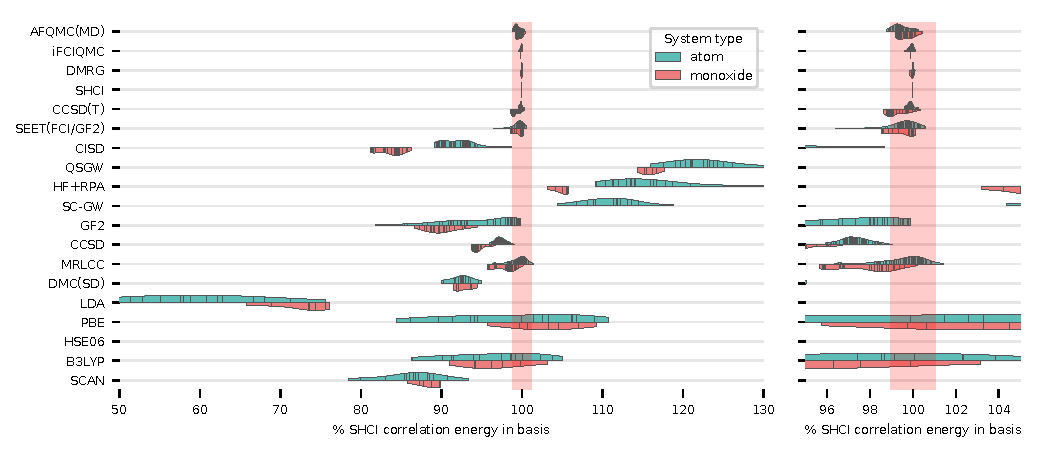
\includegraphics[width=\linewidth]{figs/correlation_energybar.pdf}
  \caption{Percent of correlation energy recovered by approximate quantum chemsitry methods, using SHCI as a reference~\cite{williams2019direct}.
}
  \label{fig:benchmark}
  \end{center}
\end{figure}

\begin{figure}
  \begin{center}
  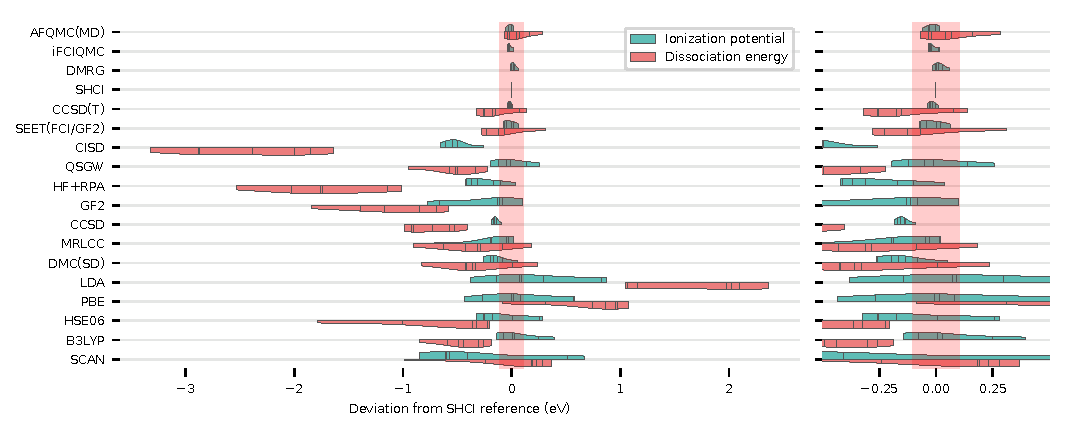
\includegraphics[width=\linewidth]{figs/BE_IP_SHCI.pdf}
  \caption{Deviation of approximate quantum chemsitry methods from SHCI reference values~\cite{williams2019direct}.
}
  \label{fig:benchmark_be}
  \end{center}
\end{figure}

We can see that all the systematic methods, including FCIQMC, DMRG, and SHCI, agree exceptionally well with each other.
This is as expected since they use the same Hamiltonian and all of these methods should give the full-CI energies without systematic errors.

However, systematic methods like these can only be applied to relatively small systems due to their high computational cost, so it is also important to study the errors in other more efficient methods.
These errors are often canceled out in previous studies when comparing to experimental data, and the results from our study make these errors directly accessible.

From these figures, we can see that both AFQMC and CCSD(T) give reasonably good agreement to the reference values and their computation costs increase much slower with the system size than the three essentially exact methods.
Other methods are much less accurate and thus may not produce reliable results for the energies.
However, they may still provide reasonably accurate results for structural optimization.

In many cases, using less accurate methods can be the only option due to the high computational cost of more accurate methods.
In such cases, benchmark results from some sample systems of similar kind can provide useful information on which approximate method to choose.
